\section{Egyszerű DNN modell felépítése}

DNN alapú rendszer esetén is az első fázis a szövegből fonéma alapú címkék előállítása, ezekről részletesebben következő fejezetben írtunk. Ezután meg kell határozni a fonémáknak a hosszát, erre egy egyszerű előrecsatolt háló alkalmas. Az idő paraméterekkel ellátott fonémákból becsülhetők az aktuális időegységre jellemző gerjesztési és spektrális paraméterek. Ezekből a paraméterekből állítható elő az eredetihez hasonló gépi hang ([4] és a BME Deep Learning előadás során elhangzottak\footnote{http://smartlab.tmit.bme.hu/oktatas-deep-learning-eloadas?eloadas=5}).

\begin{figure}[h]
	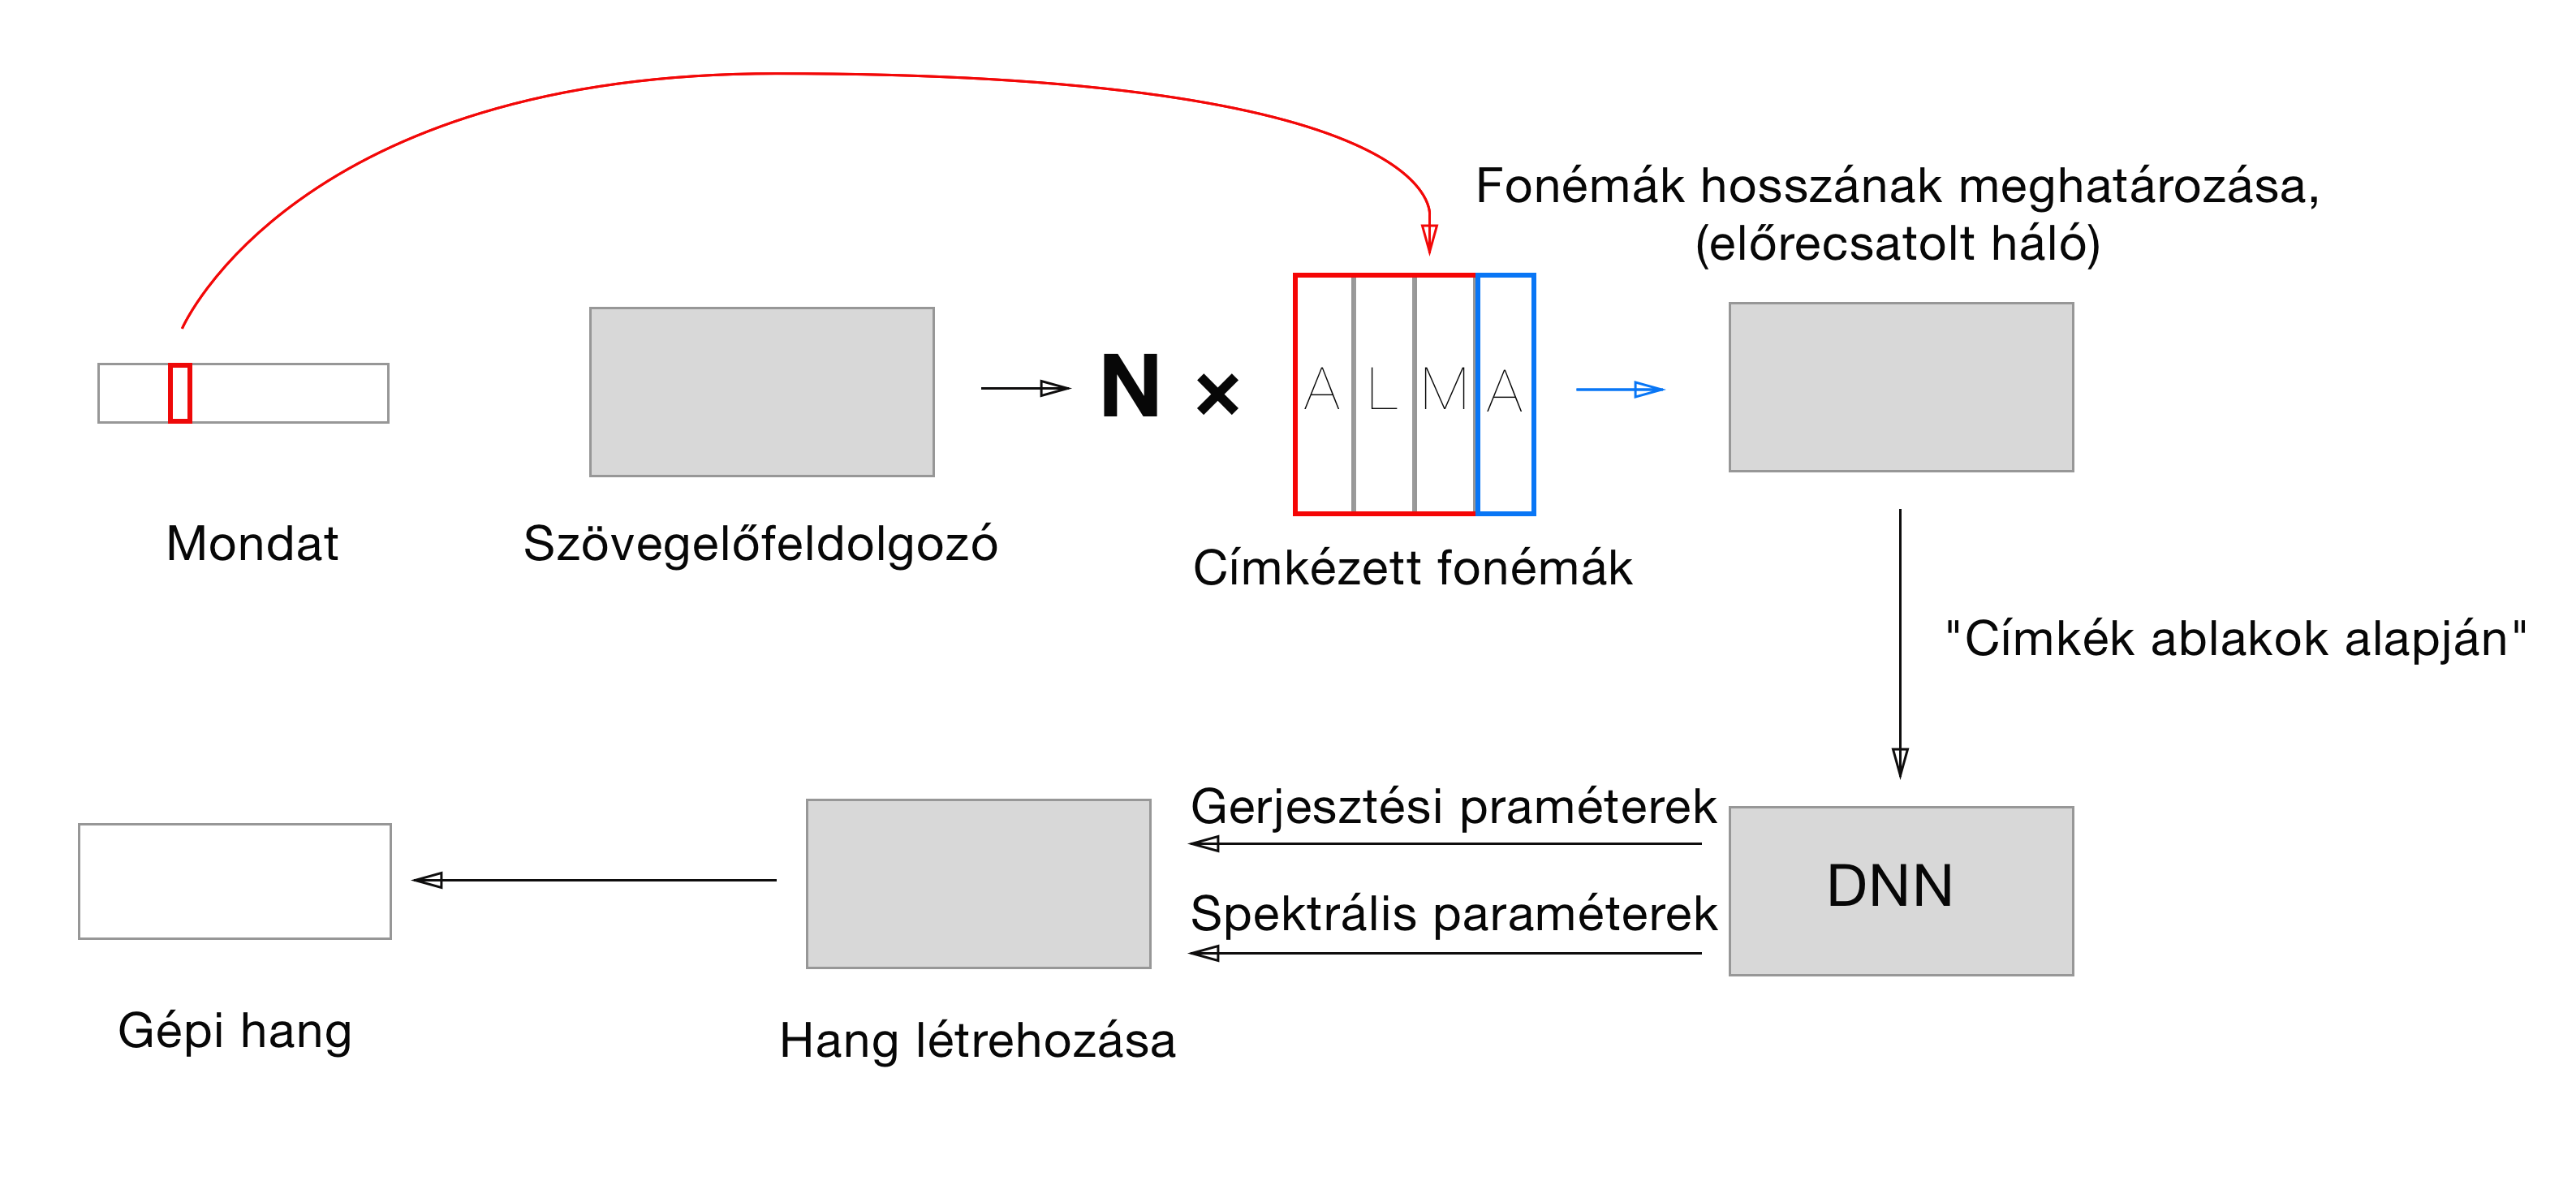
\includegraphics[width=\textwidth,keepaspectratio]{dnn_struct}
	\caption{DNN rendszer}\par\medskip\centering
\end{figure}

\subsection{Háló modellek}
Külön hálón tanítottuk a spektrális és a gerjesztési paramétereket. 

Gerjesztési paraméter problémáját két hálóra bontottuk szét. Az egyik a hang zöngésségét határozta meg a másik pedig az alapfrekvenciát, a végleges eredményeket a két háló által jósolt értékekből számítottuk ki. (Gyakorlatilag egy engedélyező jelként értelmeztünk a zöngésség értékét az alapfrekvencián.) A zöngésség meghatározása egy egyszerűbb probléma erre  egy 6 rejtett réteget, rétegenként 512 neuront tartalmazó, RELU aktivációs függvényt, SGD optimalizálást és MSE költségfüggvényt alkalmazó hálót hoztunk létre. Az alapfrekvencia becslésére 6 rejtett réteget, rétegenként 1024 neuront tartalmazó, tanh és sigmoid aktivációs függvényt, SGD optimalizációt és MSE költségfüggvényt használó hálót alkalmaztunk. Utóbbi esetén a rétegenként alkalmaztunk Dropout-ot, tanítás során pedig early stopping-ot.

A gerjesztési paramétereket meghatározó háló hasonlóan épült fel az alapfrekvenciát becslő hálóhoz.

\begin{figure}[h]
\begin{minipage}{0.45\textwidth}
	\begin{center}
		\textbf{Zöngésség meghatározása}\par\medskip
		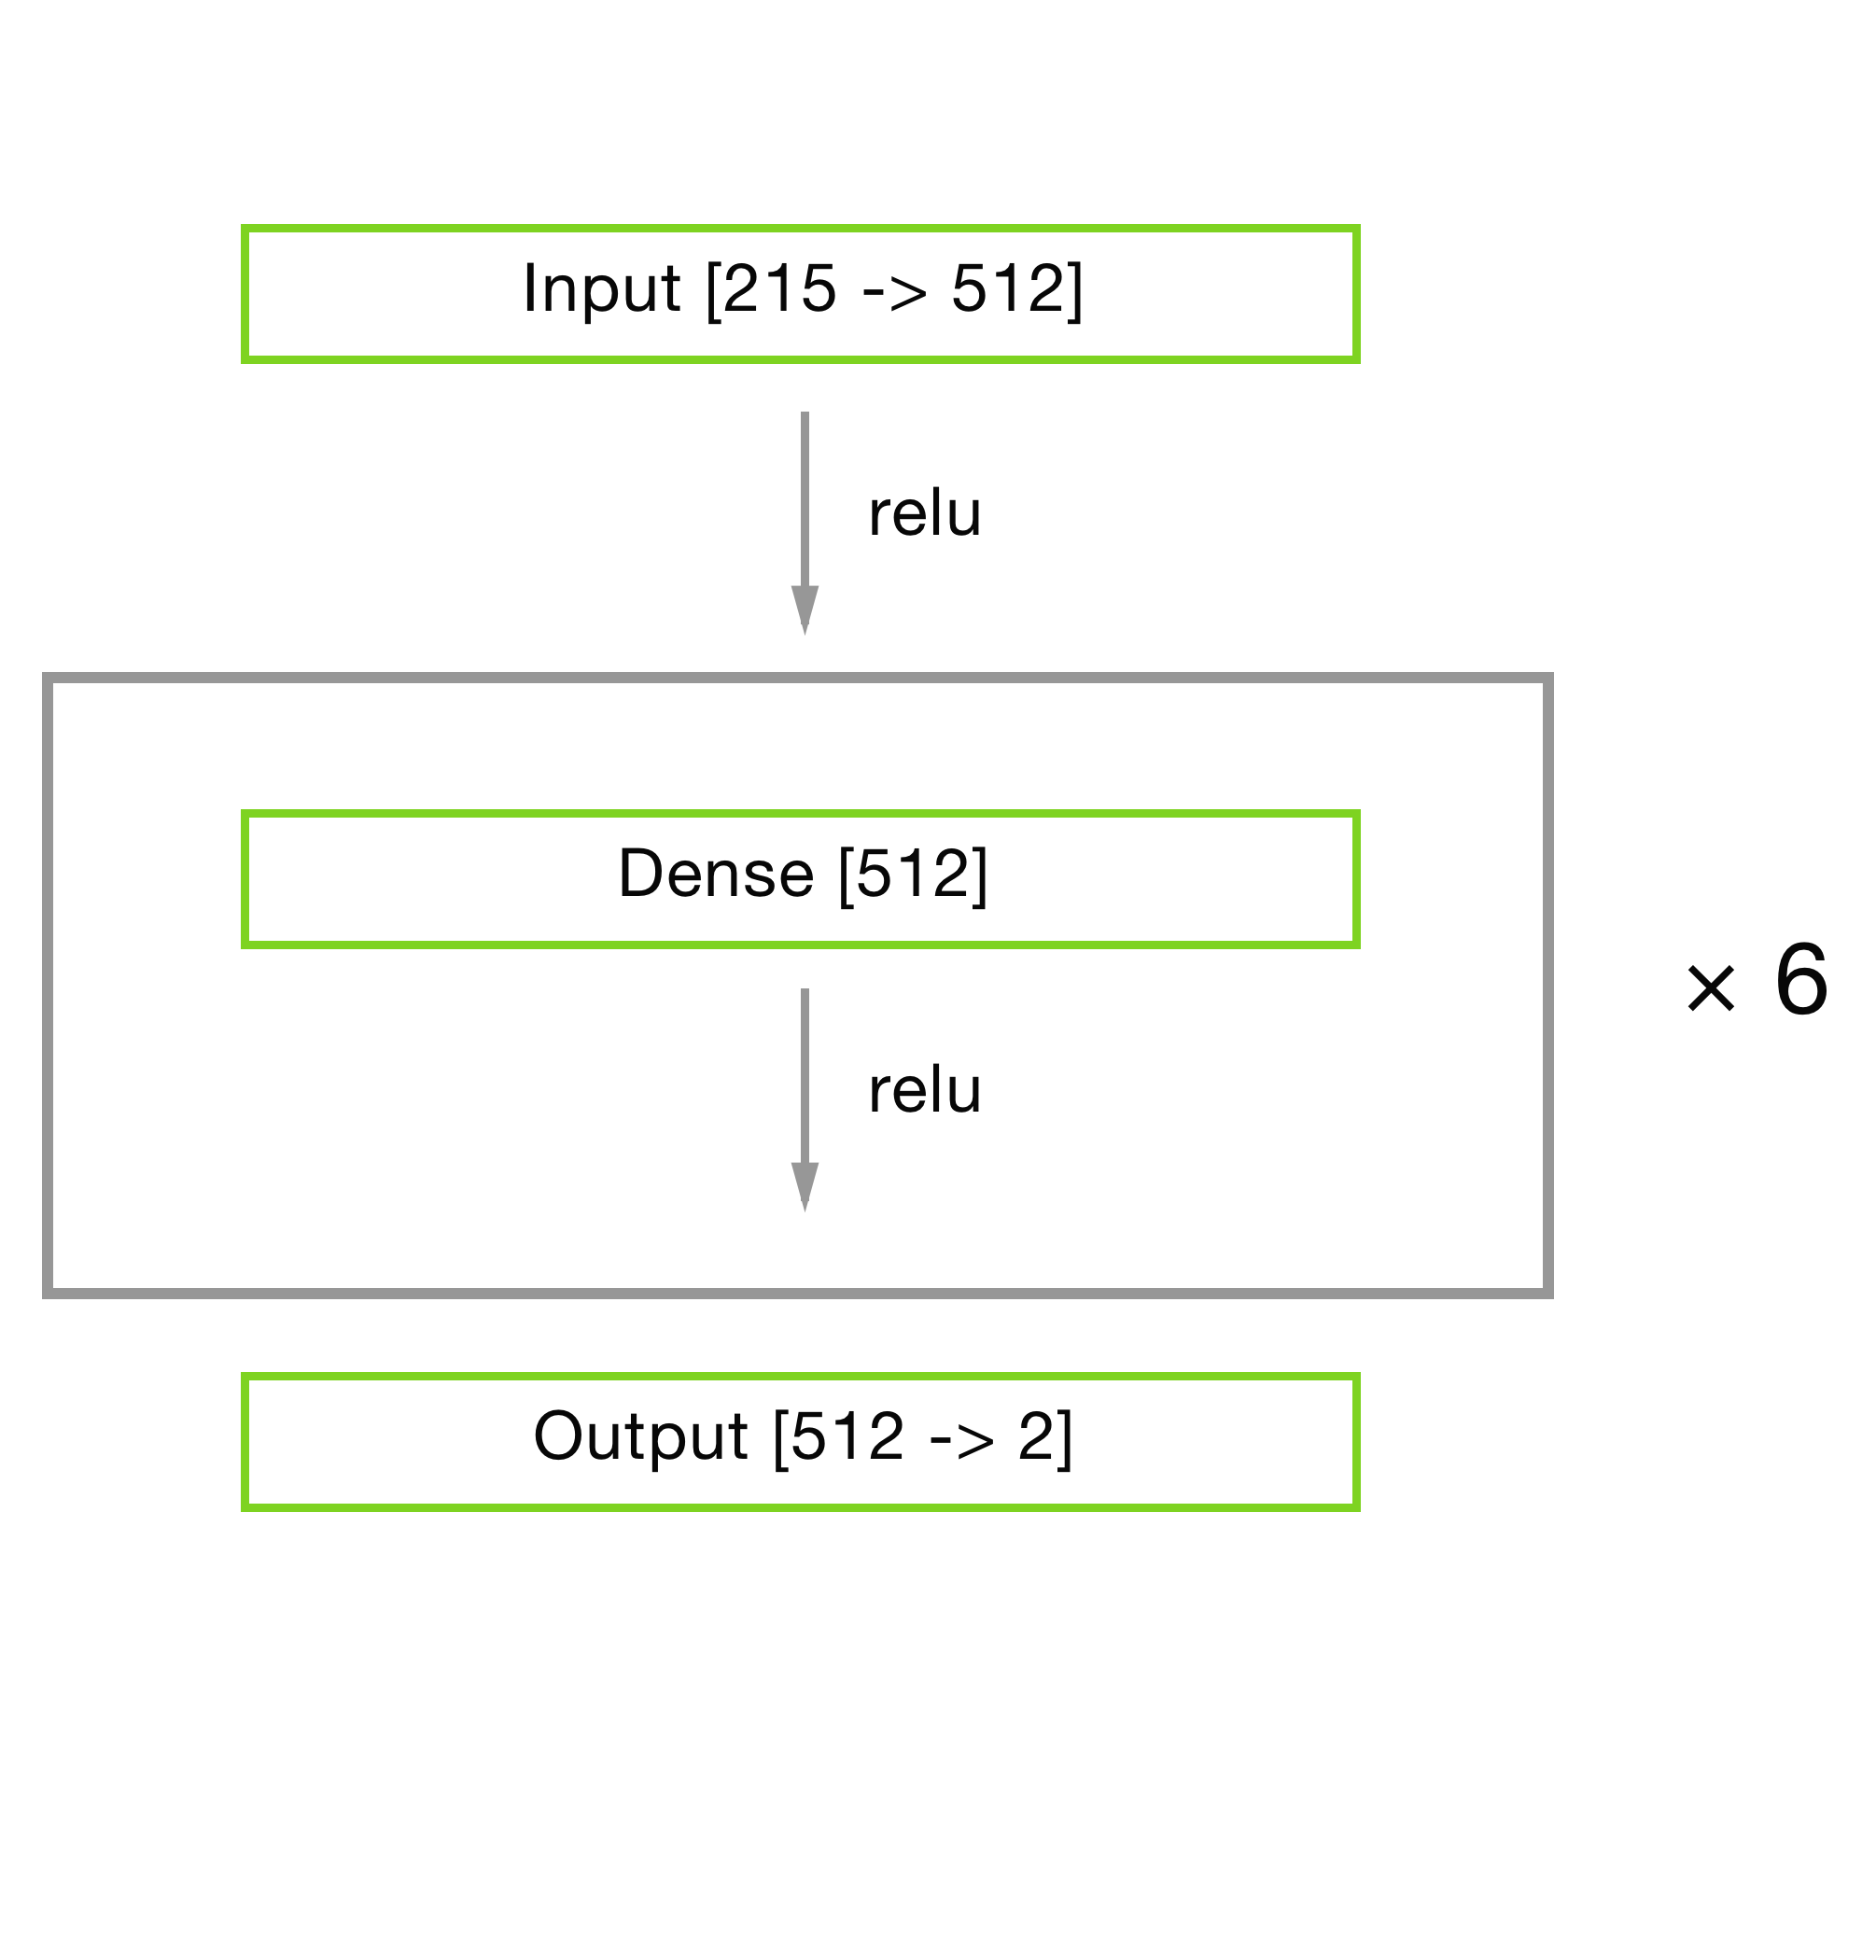
\includegraphics[width=0.6\textwidth,keepaspectratio]{vuv_net}
	\end{center}
\end{minipage}
\begin{minipage}{0.45\textwidth}
	\begin{center}
		\textbf{Alapfrekvencia meghatározása}\par\medskip
		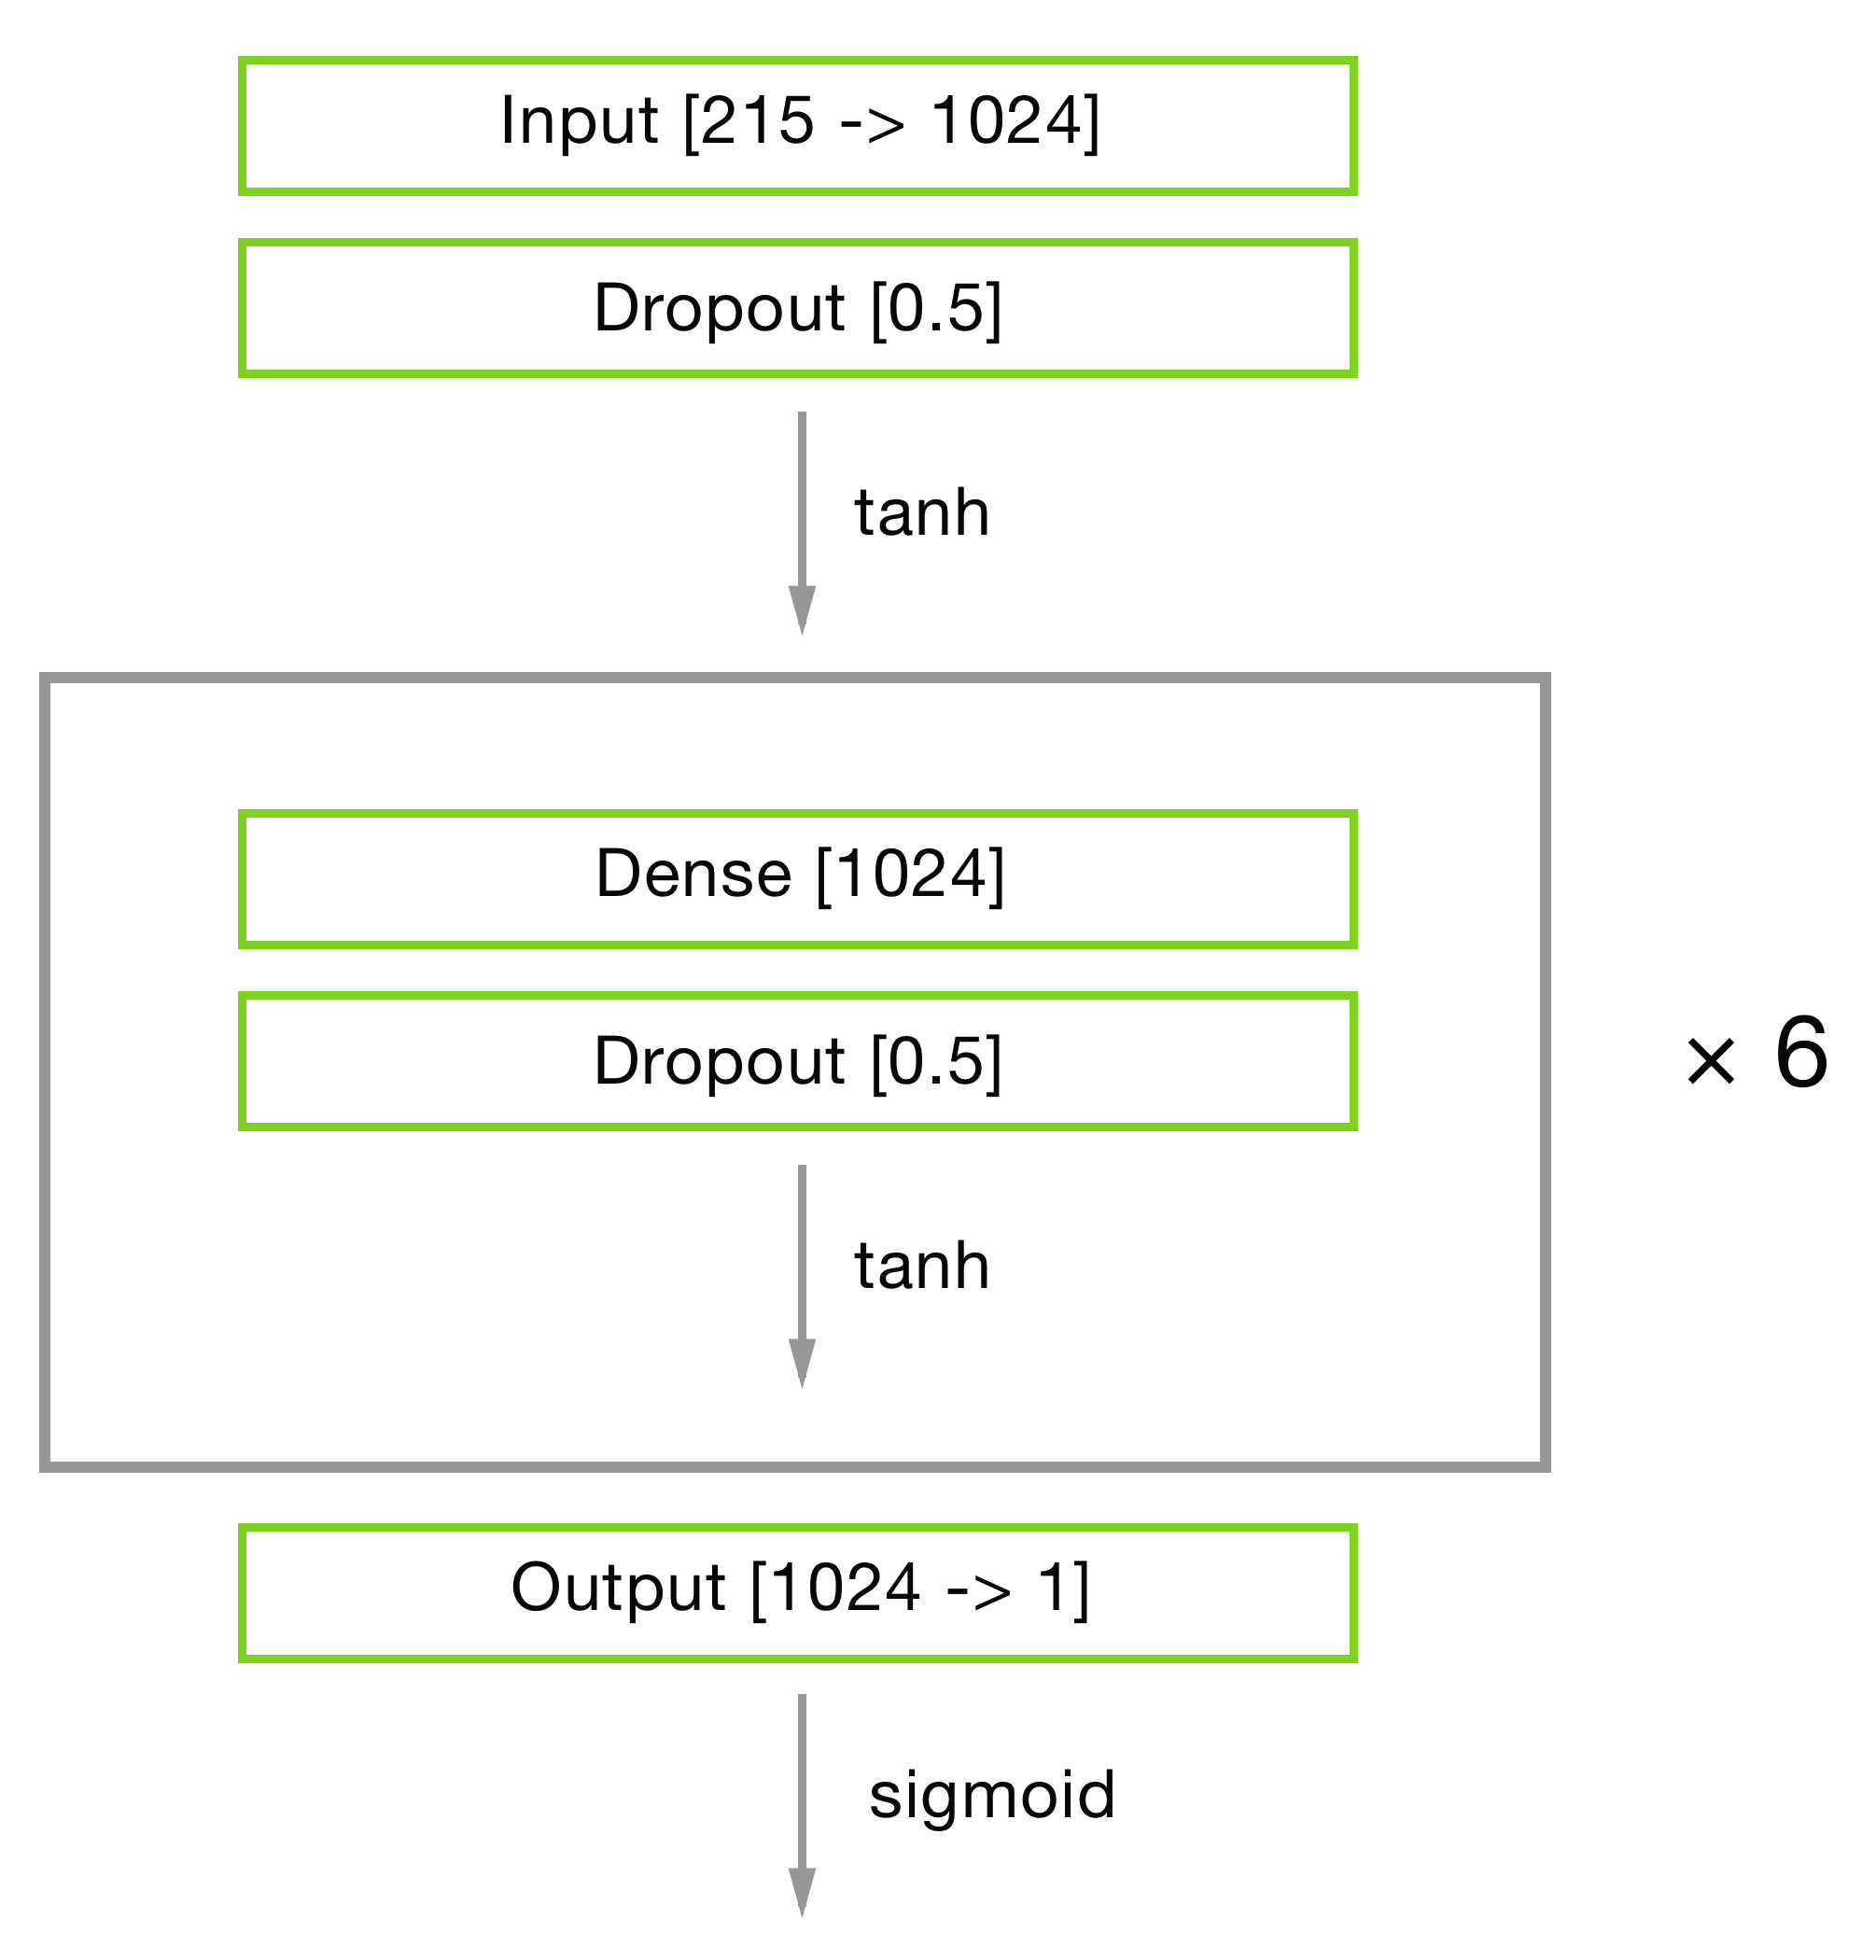
\includegraphics[width=0.6\textwidth,keepaspectratio]{pitch_net}
	\end{center}
\end{minipage}
\caption{Zöngésség és alapfrekvencia hálók}
\end{figure}
\begin{comment}
regi reszek

A továbbiakban egy DNN modell alkalmazása olvasható. A megismert címkéket továbbiakkal egészítettük ki, majd ez alapján generáltunk gerjesztési és spektrális paramétereket, amikből előállítható az audio.





Előrecsatolt mély neurális hálózatot építettünk fel, 6 rejtett réteggel, tanh és sigmoid aktivációs függvényekkel, SGD optimalizálóval és MSE költségfüggvénnyel. A háló rétegeire Dropoutot is használtunk. (/!TODO ref)
A megállást early stoppinggal detektáltuk.

/!TODO háló modell kép

\end{comment}

